\subsection{Limitations}
\label{sec:omp:limitations}
% \todo[inline]{Describe the locality problems}
% \todo[inline]{Opportunity to show here that cute image that displays locality of the mesh}

The main problem with this implemetation is data locality. While these issues are softened using a SOA approach, and the method is a first order one, the algorithm is still not very cache friendly in either of the core functions.

In \computeflux, each edge requires access to data from the two adjacent cells. While the access to edges is contiguous, access to cells is not for most of the iterations. Yet, border edges do not require the second edge.

\update on the other hand requires access to all the edges in a cell, which are always more than two. Analogously, the access to cells is contiguous, but the access to edges is not. Since there are more edges per cell than there are cells per edge, this function is most likely the bottleneck of the main loop.

The locality issues may be improved by changing how the mesh is built. The generator used for this project (\texttt{gmsh}) does not optimize the mesh locality (see \cref{fig:locality}).

\todo[inline,color=red!40]{Adicionar aqui referência ao parmetis e ao trabalho do Hoppe e explicar que optamos não arriscar o tempo com isto. Tenho sono, vou dormir.}
\todo[inline,color=green!40]{Devias tar mesmo pedrado quando escreveste esta coisa: Since each edge has more edges, than an edge has adjacent cells, and since no edge may be neglect for any cell}

\begin{figure}[!htp]
	\centering
	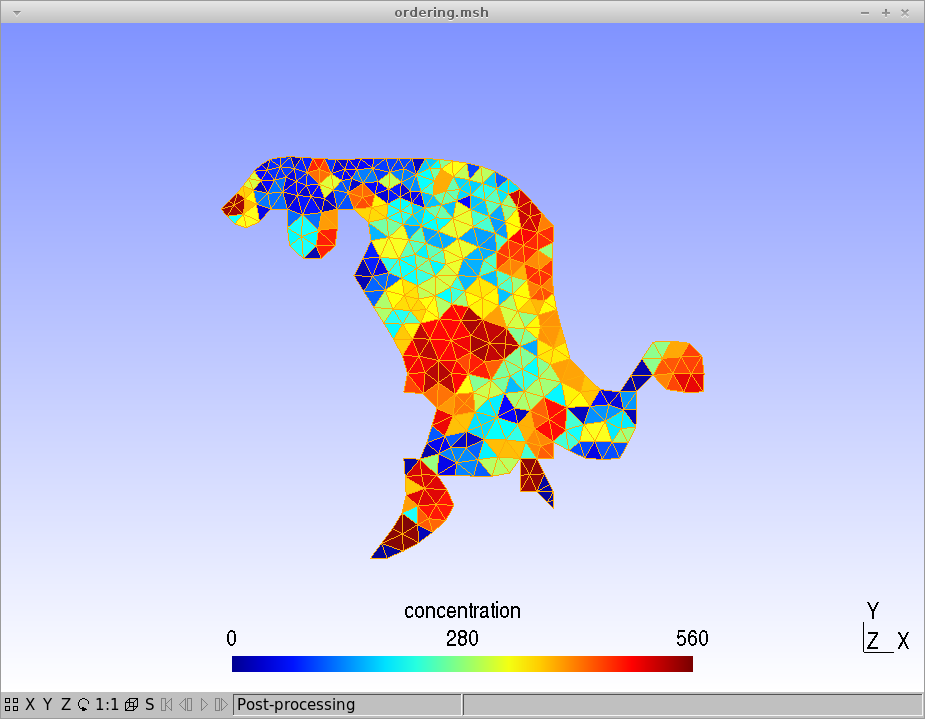
\includegraphics[width=\columnwidth]{locality_tiny.png}
	\caption{Cell locality in the mesh used as test case in this document (with increased granularity for visibility). The more different the color, the more distant the cells are in the data structure.}
	\label{fig:locality}
\end{figure}
